% !TEX root = ../ejemplo-memoria.tex
% Contenidos del capítulo.
% Las secciones presentadas son orientativas y no representan
% necesariamente la organización que debe tener este capítulo.

% Diagramas de clases, de secuencia, de despliegue, diseño de
% pantallas, etc

\section{Diseño de base de datos}

La base de datos de la aplicación está diseñada para almacenar información sobre mujeres relevantes, lugares asociados, rutas temáticas, usuarios y el historial de visitas. El diseño sigue una estructura relacional y está implementado en PostgreSQL mediante modelos definidos en Django.

\subsection{Tablas principales}

A continuación se describen las tablas principales que conforman el modelo de datos:

\begin{itemize}
    \item \textbf{AreaInvestigacion}: Tabla destinada a almacenar las distintas áreas de investigación o ámbitos destacados.
    \begin{itemize}
        \item \textbf{id} (clave primaria)
        \item \textbf{nombre}: nombre único del área.
    \end{itemize}
    \item \textbf{Mujer}: Tabla que representa a una mujer relevante en la aplicación.
    \begin{itemize}
        \item \textbf{id} (clave primaria)
        \item \textbf{nombre}
        \item \textbf{descripcion}
        \item \textbf{foto}
        \item \textbf{areas\_investigacion}: lista de cadenas de texto (\texttt{ArrayField}) con los nombres de las áreas de investigación asociadas.
        \item \textbf{fechas}: información de fechas relevantes.
    \end{itemize}
    \item \textbf{Lugar}: Tabla que representa un lugar geolocalizado relacionado con una mujer.
    \begin{itemize}
        \item \textbf{id} (clave primaria)
        \item \textbf{nombre}
        \item \textbf{descripcion}
        \item \textbf{latitud}
        \item \textbf{longitud}
        \item \textbf{foto}
        \item \textbf{ar\_url}: enlace a contenido de realidad aumentada.
        \item \textbf{mujer\_id} (clave foránea): referencia a la mujer destacada.
    \end{itemize}
    \item \textbf{Ruta}: Tabla que agrupa lugares y mujeres en recorridos temáticos.
    \begin{itemize}
        \item \textbf{id} (clave primaria)
        \item \textbf{nombre}
        \item \textbf{descripcion}
        \item Relación de tipo ManyToMany con las tablas \textbf{Mujer} y \textbf{Lugar}.
    \end{itemize}
    \item \textbf{UserProfile}: Tabla que extiende el modelo de usuario de Django con información adicional.
    \begin{itemize}
        \item \textbf{id} (clave primaria)
        \item \textbf{user\_id} (relación uno a uno con User)
        \item \textbf{birth\_date}
        \item \textbf{email}
    \end{itemize}
    \item \textbf{VisitedLugar}: Tabla que almacena el historial de lugares visitados por cada usuario.
    \begin{itemize}
        \item \textbf{id} (clave primaria)
        \item \textbf{user\_id} (clave foránea)
        \item \textbf{lugar\_id} (clave foránea)
        \item \textbf{visited\_at}: fecha y hora de la visita.
    \end{itemize}
    \item \textbf{VisitedLugarRuta}: Tabla que almacena el historial de lugares visitados por ruta y usuario.
    \begin{itemize}
        \item \textbf{id} (clave primaria)
        \item \textbf{user\_id} (clave foránea)
        \item \textbf{ruta\_id} (clave foránea)
        \item \textbf{lugar\_id} (clave foránea)
        \item \textbf{visited\_at}: fecha y hora de la visita.
    \end{itemize}
\end{itemize}

\subsection{Relaciones}

\begin{itemize}
    \item Un \textbf{Lugar} pertenece a una \textbf{Mujer}.
    \item Una \textbf{Mujer} puede tener varios \textbf{Lugares} asociados.
    \item Una \textbf{Ruta} puede incluir varias \textbf{Mujeres} y varios \textbf{Lugares} (relaciones de tipo ManyToMany).
    \item Un \textbf{UserProfile} extiende a un \textbf{User} de Django.
    \item \textbf{VisitedLugar} y \textbf{VisitedLugarRuta} permiten registrar el historial de visitas de los usuarios, tanto de lugares individuales como de lugares dentro de rutas.
\end{itemize}

\subsection{Esquema de tablas}

El siguiente esquema resume la estructura de las tablas principales de la base de datos:

\begin{verbatim}
Mujer             (id, nombre, descripcion, foto, areas_investigacion, fechas)
Lugar             (id, nombre, descripcion, latitud, longitud, foto, ar_url, mujer_id)
Ruta              (id, nombre, descripcion)
UserProfile       (id, user_id, birth_date, email)
VisitedLugar      (id, user_id, lugar_id, visited_at)
VisitedLugarRuta  (id, user_id, ruta_id, lugar_id, visited_at)
AreaInvestigacion (id, nombre)
\end{verbatim}

\subsection{Justificación del diseño}

El modelo de datos relacional implementado garantiza la integridad y la eficiencia en las consultas. El historial de visitas se almacena en tablas separadas, lo que permite la obtención de estadísticas y la personalización de la experiencia del usuario.

\begin{figure}[H]
    \centering
    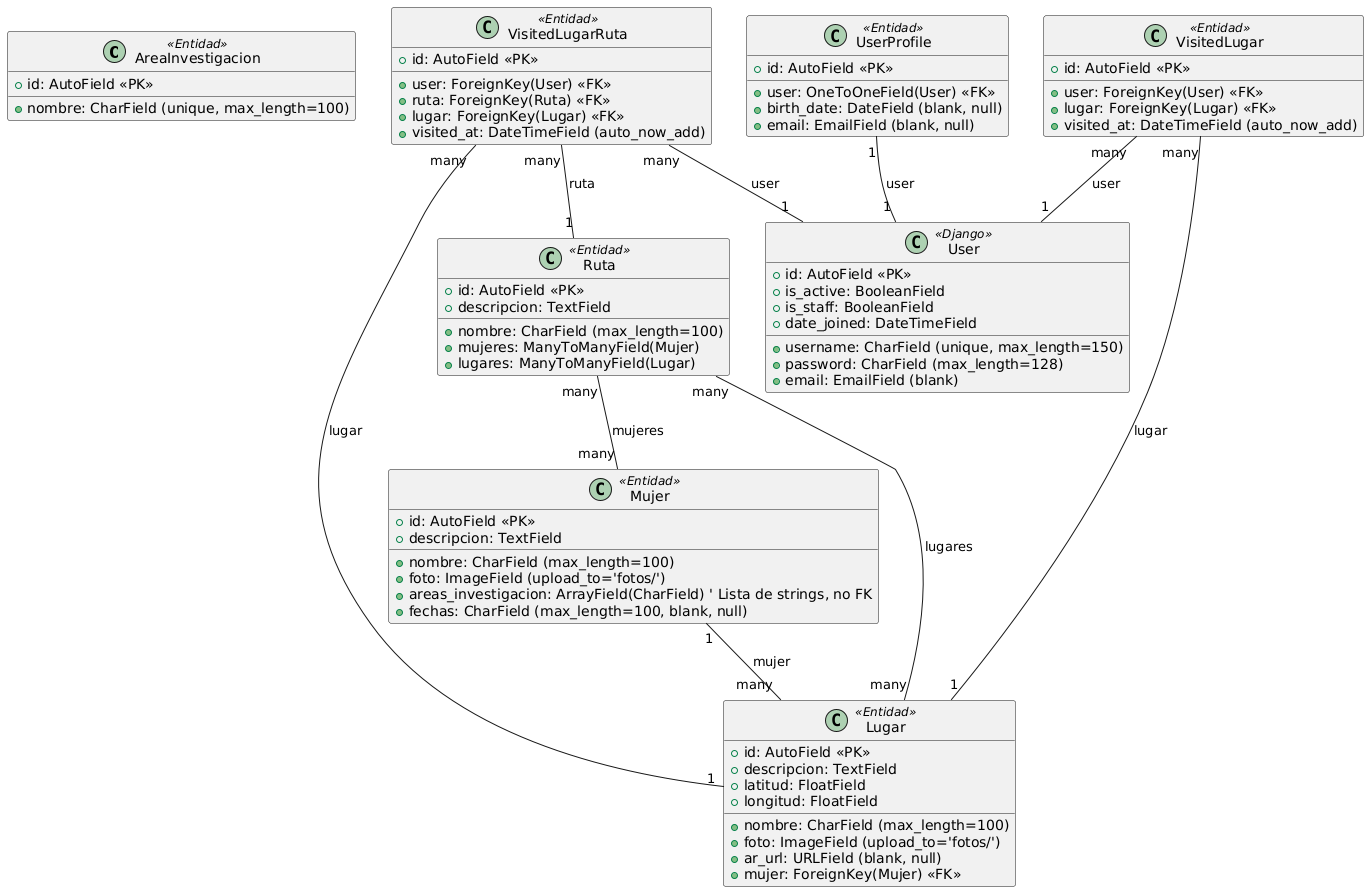
\includegraphics[width=1\textwidth]{figs/diagrama_clases.png}
    \caption{Diagrama de clases y tablas principales de la base de datos}
\end{figure}